\section{SIDEWAYS PICTURES}
Figures can be rotated as shown in Figure~\ref{fig:sideways}  a landscape mode using the \texttt{rotating} package. A package for rotated objects in LATEX
Robin Fairbairns, Sebastian Rahtz, Leonor Barroca.


The code uses the \verb!sideways! environment. In this particular example, we use footnotes, in the caption and hence we add some code to achieve this.  Note that the package defaults take care of verso and recto page display so that you do not need to   worry about rotating the image clockwise or counterclockwise. The package rotates by default clockwise.

\begin{tcolorbox}
\begin{lstlisting}
\begin{sidewaysfigure}

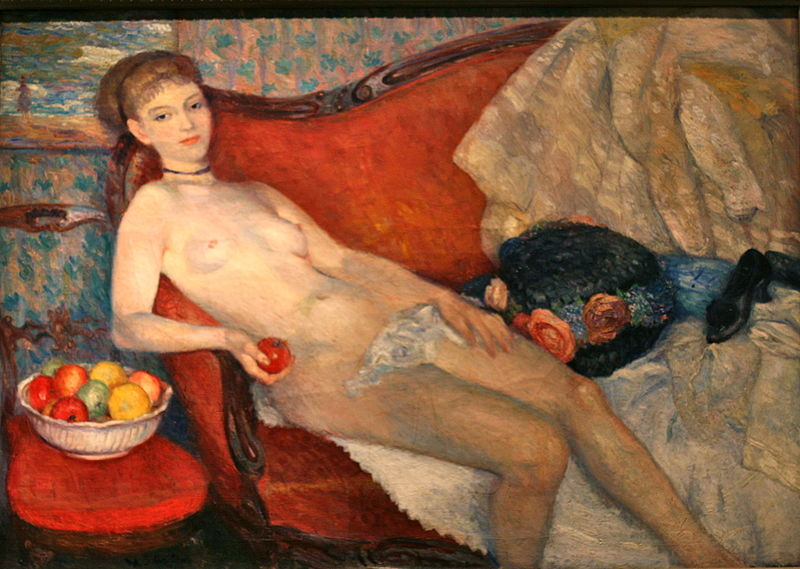
\includegraphics[height=0.5\textheight, width=0.9\textwidth, keepaspectratio]{nudewithapple}
\captionof{figure}{The package sets the\protect\footnotemark[1] footnotes\protect\footnotemark[2] of a single-column document in two columns;
the package offers a range of parameters to determine\protect\footnotemark[3] the exact appearance\protect\footnotemark[4] of the two columns.}
\vspace{3\baselineskip}
\footnoterule\footnotesize
\begin{minipage}[t]{0.4\linewidth}
\textsuperscript{1} This is the first footnote. And here comes some nonsense text
                    to show that the linebreaks works \par
\textsuperscript{2} This is the second footnote.\par
\end{minipage}\hfill
\begin{minipage}[t]{0.4\linewidth}
\textsuperscript{3} This is the third footnote. \par
\textsuperscript{4} This is the fourth footnote.\par
\textsuperscript{5} This is the fourth footnote.\par
\textsuperscript{6} See \url{http://tex.stackexchange.com/questions/8174/how-to-achieve-a-multi-column-layout-for-footnotes}\par
\end{minipage}
\end{sidewaysfigure}
\end{lstlisting}
\end{tcolorbox}


\begin{sidewaysfigure}

\centering
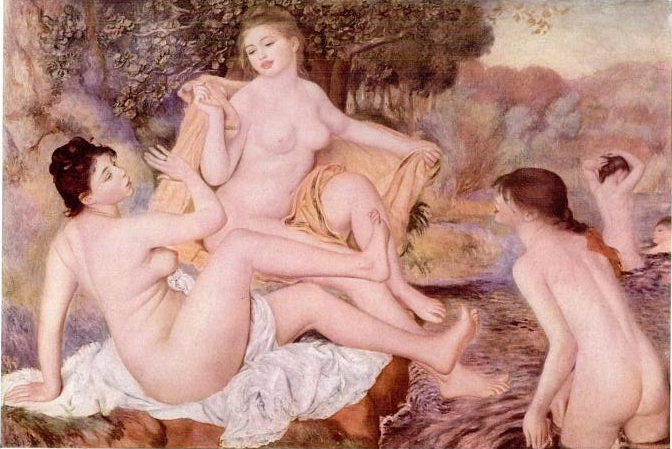
\includegraphics[height=0.5\textheight, width=0.9\textwidth, keepaspectratio]{bathers-01}
\captionof{figure}{The package sets the\protect\footnotemark[1] footnotes\protect\footnotemark[2] of a single-column document in two columns;
the package offers a range of parameters to determine\protect\footnotemark[3] the exact appearance\protect\footnotemark[4] of the two columns.}
\vspace{3\baselineskip}
\footnoterule\footnotesize
\begin{minipage}[t]{0.49\linewidth}
\textsuperscript{1} This is the first footnote. And here comes some nonsense text
                    to show that the linebreaks works \par
\textsuperscript{2} This is the second footnote.\par
\end{minipage}\hfill
\begin{minipage}[t]{0.49\linewidth}
\textsuperscript{3} This is the third footnote. \par
\textsuperscript{4} This is the fourth footnote.\par
\textsuperscript{5} This is the fourth footnote.\par
\textsuperscript{6} See \url{http://tex.stackexchange.com/questions/8174/how-to-achieve-a-multi-column-layout-for-footnotes}\par
\end{minipage}
\end{sidewaysfigure}


\begin{sidewaysfigure}

\centering
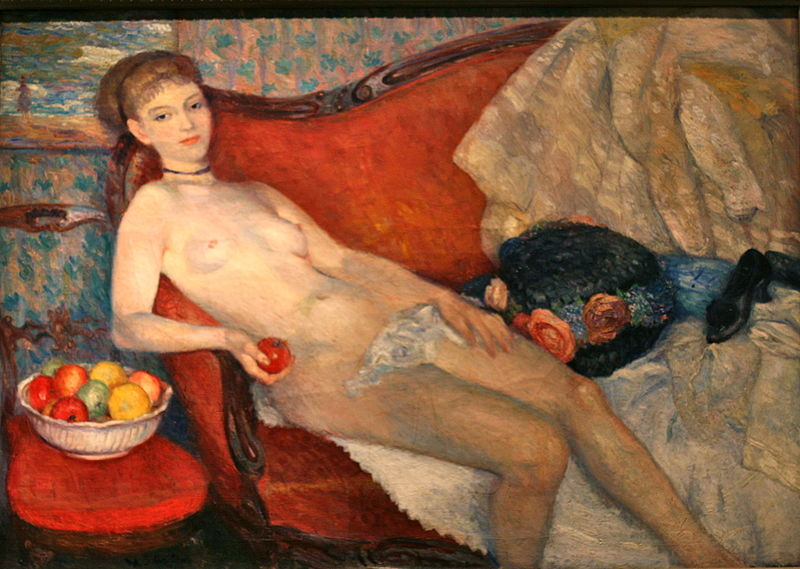
\includegraphics[height=0.5\textheight, width=0.9\textwidth, keepaspectratio]{nudewithapple}
\captionof{figure}{The package sets the\protect\footnotemark[1] footnotes\protect\footnotemark[2] of a single-column document in two columns;
the package offers a range of parameters to determine\protect\footnotemark[3] the exact appearance\protect\footnotemark[4] of the two columns.}
\vspace{3\baselineskip}
\footnoterule\footnotesize
\begin{minipage}[t]{0.49\linewidth}
\textsuperscript{1} This is the first footnote. And here comes some nonsense text
                    to show that the linebreaks works \par
\textsuperscript{2} This is the second footnote.\par
\end{minipage}\hfill
\begin{minipage}[t]{0.49\linewidth}
\textsuperscript{3} This is the third footnote. \par
\textsuperscript{4} This is the fourth footnote.\par
\textsuperscript{5} This is the fourth footnote.\par
\textsuperscript{6} See \url{http://tex.stackexchange.com/questions/8174/how-to-achieve-a-multi-column-layout-for-footnotes}\par
\end{minipage}
\end{sidewaysfigure}




\clearpage

\begin{figure}

\centering
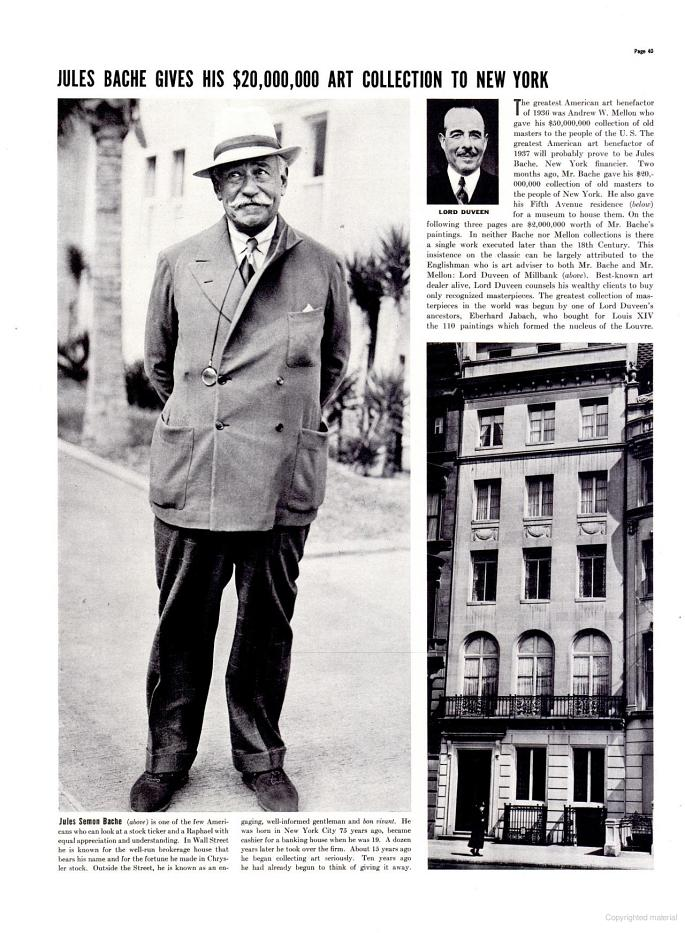
\includegraphics[height=\textheight, width=\textwidth, keepaspectratio]{julesbache}
\end{figure}

\begin{figure}

\centering
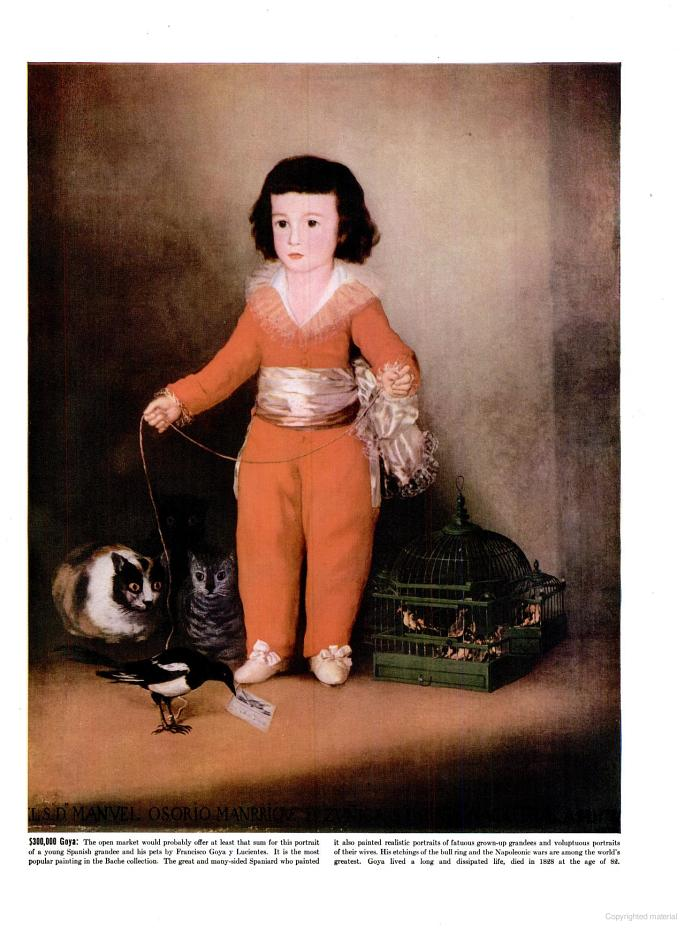
\includegraphics[height=\textheight, width=\textwidth, keepaspectratio]{goya01}
\end{figure}

\begin{figure}

\centering
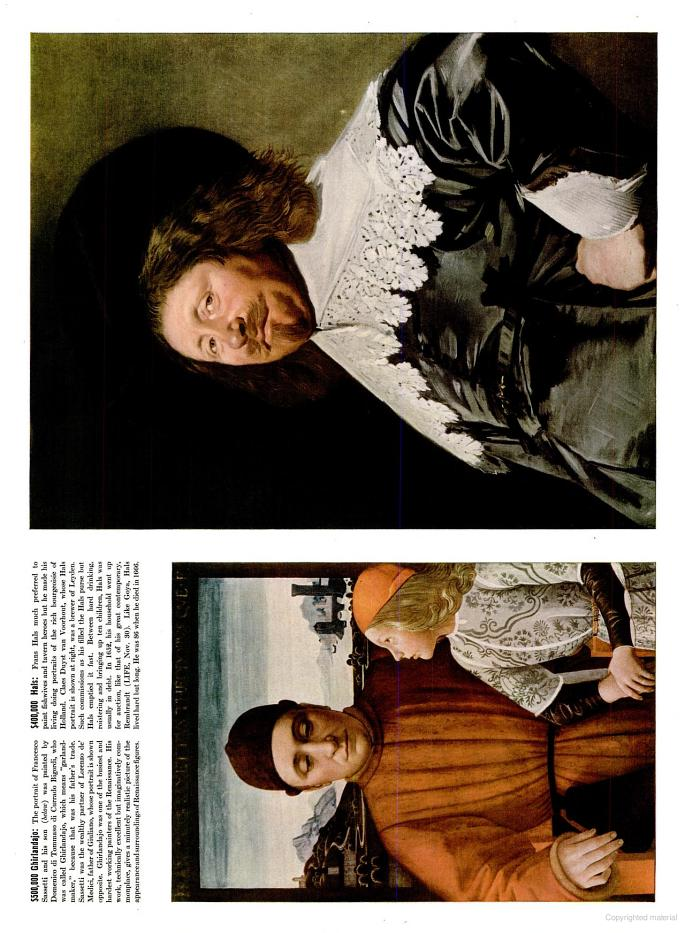
\includegraphics[height=\textheight, width=\textwidth, keepaspectratio]{goya-sideways}
\end{figure}

\begin{figure}

\centering
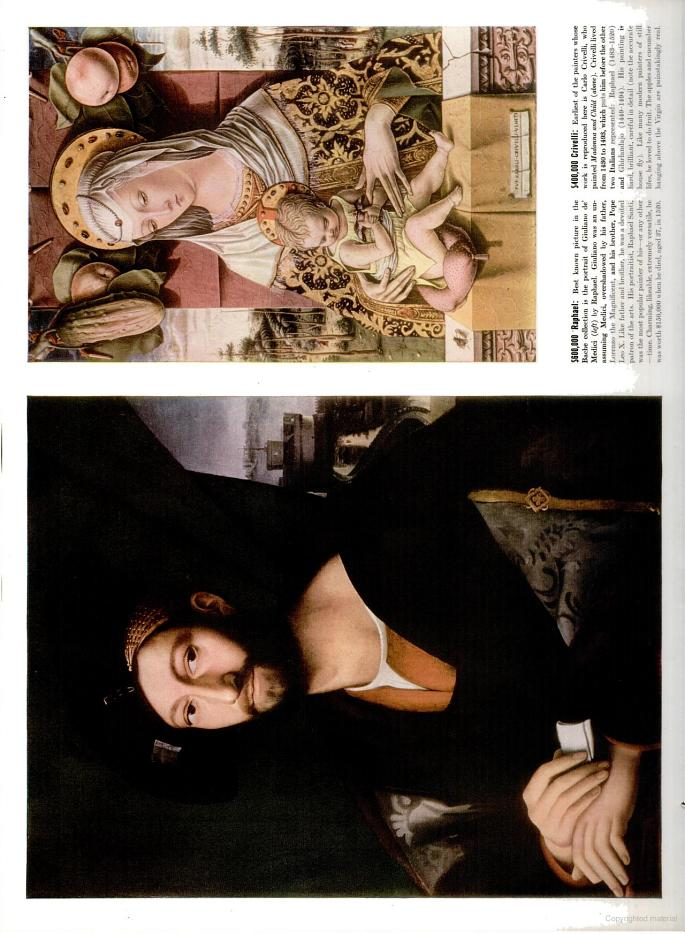
\includegraphics[height=\textheight, width=\textwidth, keepaspectratio]{goya-sideways01}
\end{figure}

\pagebreak






